\documentclass[12pt, a4paper]{report}
\usepackage[top=1cm, left=1cm, right=1cm]{geometry}

\usepackage[utf8]{inputenc}
\usepackage[russian]{babel}

\usepackage{array}
\newcolumntype{M}[1]{>{\centering\arraybackslash}m{#1}}

\usepackage{hyperref}
\hypersetup{
	colorlinks,
	citecolor=black,
	filecolor=black,
	linkcolor=black,
	urlcolor=black
}

\usepackage{sectsty}
\allsectionsfont{\centering}

\usepackage{indentfirst}
\setlength\parindent{24pt}

\usepackage{algorithm}
\usepackage[noend]{algpseudocode}

\usepackage{listings}
\usepackage{xcolor}
\definecolor{codegreen}{rgb}{0,0.6,0}
\definecolor{codegray}{rgb}{0.5,0.5,0.5}
\definecolor{codepurple}{rgb}{0.58,0,0.82}
\definecolor{backcolour}{rgb}{0.95,0.95,0.92}
\lstdefinestyle{mystyle}{
    backgroundcolor=\color{backcolour},   
    commentstyle=\color{codegreen},
    keywordstyle=\color{magenta},
    numberstyle=\normalsize\color{codegray},
    stringstyle=\color{codepurple},
    basicstyle=\ttfamily\footnotesize,
    breakatwhitespace=false,         
    breaklines=true,                 
    captionpos=b,                    
    keepspaces=true,                 
    numbers=left,                    
    numbersep=5pt,                  
    showspaces=false,                
    showstringspaces=false,
    showtabs=false,                  
    tabsize=2
}

\usepackage{graphicx}
\graphicspath{{plots/pictures/}}

\begin{document}
	\begin{titlepage}
		\begin{center}
			\large \textbf{Министерство науки и высшего образования Российской Федерации} \\
			\large \textbf{Федеральное государственное бюджетное образовательное учреждение высшего образования} \\
			\large \textbf{«Российский химико-технологический университет имени Д.И. Менделеева»} \\

			\vspace*{4cm}
			\LARGE \textbf{ОТЧЕТ ПО ЛАБОРАТОРНОЙ РАБОТЕ №3}

			\vspace*{4cm}
			\begin{flushright}
				\Large
				\begin{tabular}{>{\raggedleft\arraybackslash}p{9cm} p{10cm}}
					Выполнил студент группы КС-36: & Золотухин А.А. \\
					Ссылка на репозиторий: & https://github.com/ \\
					& MUCTR-IKT-CPP/ \\
					& ZolotukhinAA\_36\_ALG \\
					Принял: & Крашенников Роман Сергеевич \\
					Дата сдачи: & 10.03.2025 \\
				\end{tabular}
			\end{flushright}

			\vspace*{6cm}
			\Large \textbf{Москва \\ 2025}
		\end{center}
	\end{titlepage}

	\tableofcontents
	\thispagestyle{empty}
	\newpage

	\pagenumbering{arabic}

	\section*{Описание задачи}
	\addcontentsline{toc}{section}{Описание задачи}
	\large
	Написать свою реализацию двусвязного списка:
	\begin{itemize}
		\item добавление элемента в начало, в конец, в произвольное место;
		\item удаление элемента из списка.
	\end{itemize}
	\par
	В рамках лабораторной работы необходимо изучить и реализовать двусвязный список. Структура должна:
	\begin{itemize}
		\item использовать шаблонный подход, обеспечивая работу контейнера с произвольными данными;
		\item реализовывать своё итератор, предоставляющий стандартный для языка механизм работы с ним (для \textit{C++} это операции \textit{++} и \textit{!=});
		\item обеспечивать работу стандартных библиотек и конструкции \textit{for each}, если она есть в языке, если их нет, то реализовать собственную функцию, использующую итератор;
		\item обеспечивать проверку на пустоту и подсчёт количества элементов.
	\end{itemize}
	\par
	Для демонстрации работы структуры необходимо создать набор тестов (под тестом понимается функция, которая создаёт структуру, проводит операцию или операции над структурой и удаляет структуру):
	\begin{itemize}
		\item заполнение контейнера \underline{1000} целыми числами в диапазоне от \underline{-1000} до \underline{1000} и подсчёт их суммы, среднего, минимального и максимального;
		\item провести проверку работы операций вставки и изъятия элементов на коллекции из \underline{10} строковых элементов;
		\item заполнение контейнера \underline{100} структур, содержащих фамилию, имя, отчество и дату рождения (от \underline{01.01.1980} до \underline{01.01.2020}). Значения каждого поля генерируются случайно из набора заранее заданных. После заполнения необходимо найти всех людей младше \underline{20} лет и старше \underline{30} и создать новые структуры, содержащие результат фильтрации, проверить выполнение на правильность подсчётом количества элементов, не подходящих под условие в новых структурах.
	\end{itemize}
	\par
	Тесты:
	\begin{enumerate}
		\item перемешать все элементы;
		\item выполнить серию тестирования сортировки из первой лабораторной на реализованном списке и сравнить производительность с полученной на массиве.
	\end{enumerate}

	\section*{Описание метода/модели}
	\addcontentsline{toc}{section}{Описание метода/модели}
	\large

	\section*{Выполнение задачи}
	\addcontentsline{toc}{section}{Выполнение задачи}

	\newpage
	\vfill

	\begin{figure}
		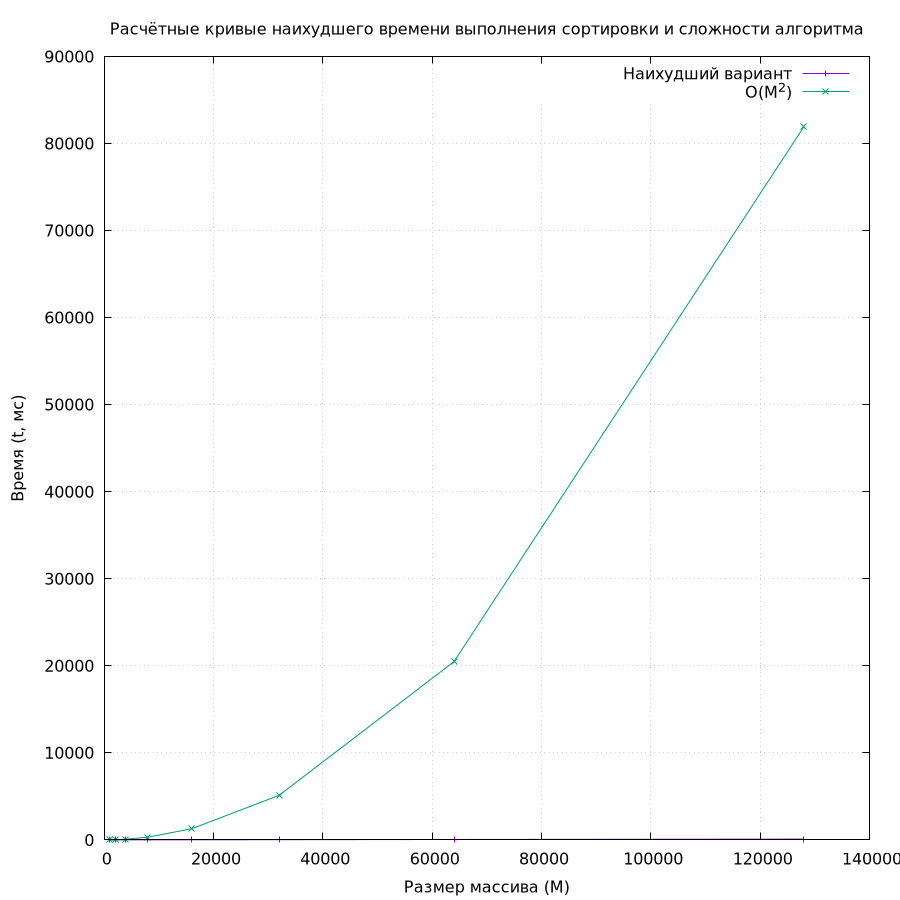
\includegraphics[width=300pt]{worst_and_complexity.png}
	\end{figure}
	\begin{figure}
		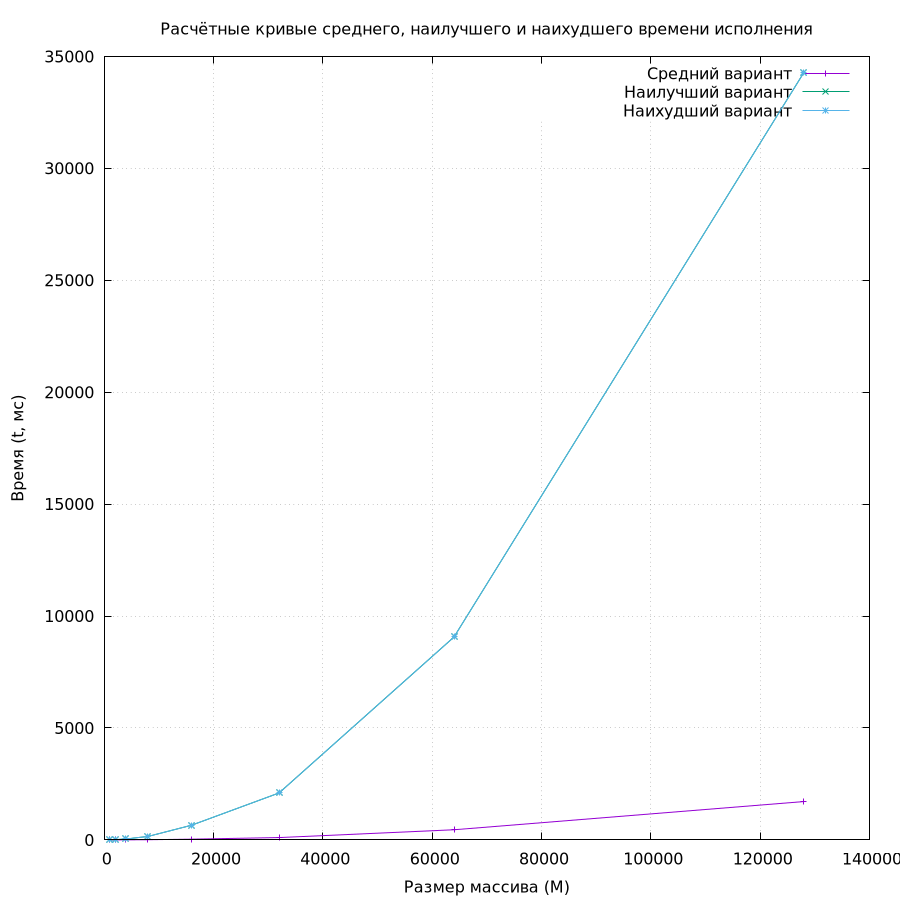
\includegraphics[width=300pt]{average_best_worst.png}
	\end{figure}
	\begin{figure}
		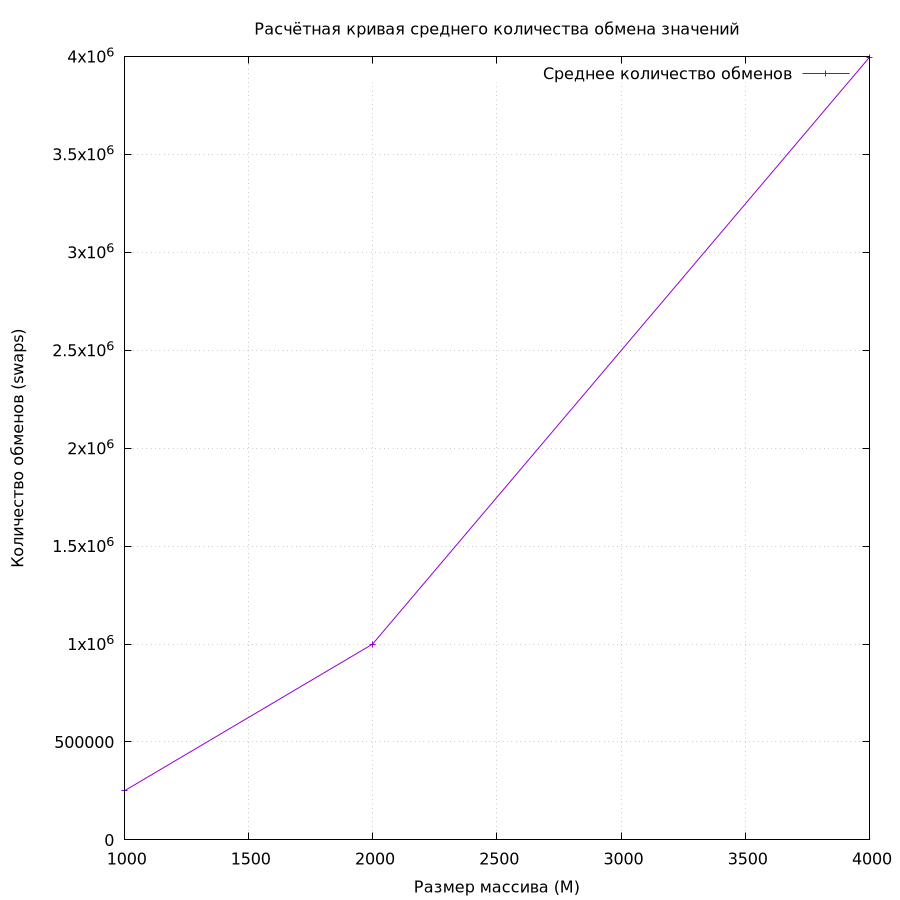
\includegraphics[width=300pt]{average_swaps.png}
	\end{figure}
	\begin{figure}
		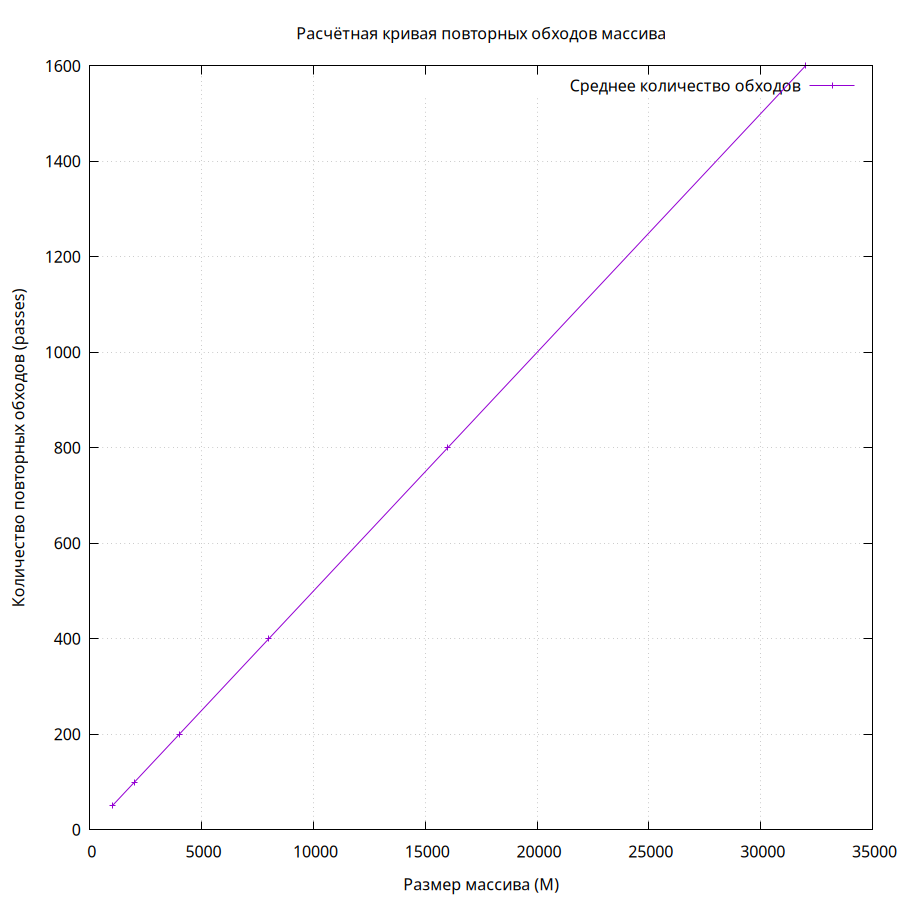
\includegraphics[width=300pt]{average_passes.png}
	\end{figure}

	\vfill
	\clearpage
	
	\section*{Выводы}
	\addcontentsline{toc}{section}{Выводы}

\end{document}
